\documentclass[10pt, a4j, dvipdfmx]{jarticle}
\usepackage{titlesec}
\usepackage[dvipdfmx]{graphicx}
\usepackage{float}
\usepackage{wrapfig}
\usepackage{subfigure}
\usepackage{caption}

\makeatletter
\newcommand{\figcaption}[1]{\def\@captype{figure}\caption{#1}}
\newcommand{\tblcaption}[1]{\def\@captype{table}\caption{#1}}
\makeatother

\title{ディジタル回路I}
\author{4年 電子システム工学科 40番  山地 駿徹}

\begin{document}
\section{目的}
集積化されたNAND回路の動作原理をよく理解し,これを用いて波形整形回路,遅延用単安定回路を組み立て,その動作原理,特性等を理解する.
本実験課題で組立てる回路パルス発生回路の前段部である.


\section{原理(実験で制作する回路の説明)}

\subsection{パルス回路の総合図}
図1にパルス発生回路の総合図を示す.波形整形回路(Schmitt回路),単安定回路A(Delay回路),単安定回路B(パルス幅決定回路),増幅回路,減衰回路,同期用信号出力回路からなっている.
\begin{figure}[H]
	\centering
	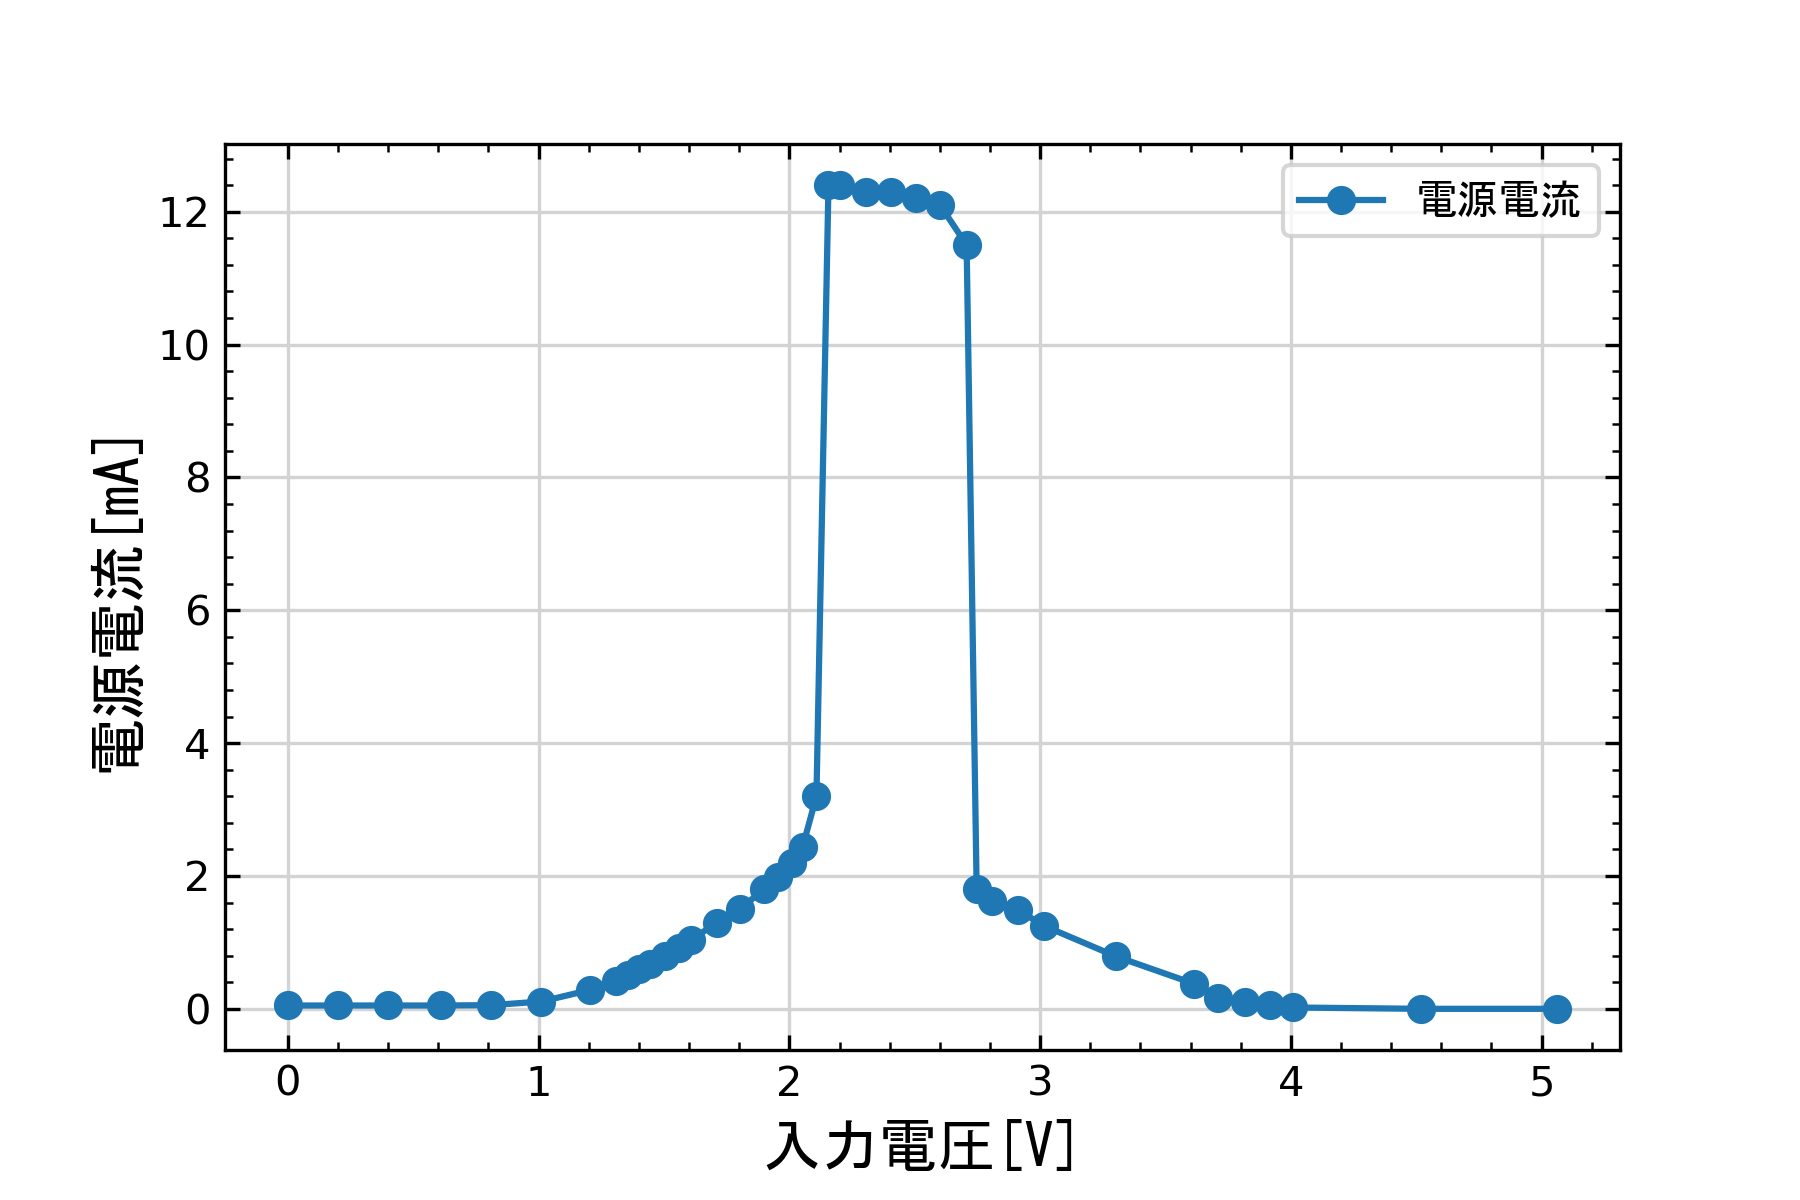
\includegraphics[height=80mm]{"D:/Document/4ES工学実験/ディジタル回路2/images/Experiment/実験3_1.png"}
	\caption{パルス発生回路}
\end{figure}
\subparagraph{パルス発生回路の入力信号}
図1に示すパルス発生回路の最初の回路である波形整形回路(Schmitt回路)の入力信号には,備品の発振器の出力信号を用いる.出呂波形は正弦波とし,周波数は1kHzを基準とする.

\subsection{NAND回路を2個つないだときの入出力特性}
図2のようにNAND回路を2個つなぎ,入力側の1端子を IC端子の$V_{CC}$用電源$+5V$につなぎ,他端子に可変電流電源を接続して入力でなんつを変化していったときの出力端子の電圧の変化を図のように電子電圧計で測定すると図3のような入出力特性がえられる.


\section{実験方法と実験結果の処理}

\subsection{波形整形回路(Schmitt回路)の静特性の測定}
波形整形回路(Schmitt回路)を,図4の構成により図2の入出力特性の測定と同様,入力の可変電流電源を変化して行ったときの出力電圧の変化すなわち静的な入出力特性を測定する.
図5のような入出力特性(ヒステリシス特性)が得られる.
ヒステリシス特性がどのように変化するか調べる.

\subsection{波形整形回路(Schmitt)の動特性の測定}
図6の構成により,入力信号として発振器により発振周波数1kHzの正弦波を入力し波形整形回路(Schmitt回路)のa,b,c,d各店の波形をオシロスコープで測定する.
図7は正弦波形の入力に対する各部の波形例を示す.測定する時,各店波形の時間軸を必ず揃えておくこと.
さらに,各点の波形は直流で観測すること.
\subparagraph{同期用信号出力機}
図6の波形整形回路(Schmitt回路)の出力を微分し,それをNAND回路に入れ,その出力を単安定回路A(Delay回路)の入力として,さらに同期用信号としても用いる.
単安定回路A(Delay回路)の出力信号を同期信号でトリガをかけ,オシロスコープで観測する.
このようにすると,同期用信号が観測しようとする単安定回路A(Delay回路)の出力より時間的に先に存在するので,単安定回路A(Delay回路)の出力の様子を確実に観測できる.

\subsection{遅延回路A(Delay回路)の遅延時間の測定}
図8のような回路を組み立てて容量C'を適当に変えて遅延時間を測定する.
図9にオシロスコープの画面例を,図10に測定結果の一例を示す.
ただし,発振器の周波数は$1kHz$および$10kHz$の2種類を測定すること.
測定終了後は,次の実験'''ディジタル回路3'で利用するため,遅延時間が$0.01[ms]$となるように容量C'を決定し,回路を変更しておくこと.


\section{実験結果}
\subsection{波形整形回路(Schmitt回路)の静特性の測定}

\section{考察}

\section{吟味事項}

\section{感想}

\section{参考文献}


\end{document}